\documentclass[12pt]{report}
\usepackage[margin=1in]{geometry}
\usepackage{amsmath,amssymb,amsthm}
\usepackage{booktabs}
\usepackage{graphicx}
\usepackage{hyperref}
\usepackage{xcolor}
\usepackage{caption}
\usepackage{enumitem}
\usepackage{tikz}
\usepackage{natbib}
\usepackage{multirow}
\usepackage{seqsplit}
\usepackage{fancyhdr}
\usepackage{setspace}
\usetikzlibrary{shapes.geometric,arrows.meta,positioning,fit,backgrounds,trees}

\newcommand{\N}{\mathcal{N}}
\newcommand{\V}{\mathcal{V}}
\newcommand{\E}{\mathcal{E}}
\DeclareMathOperator*{\argmin}{arg\,min}
\DeclareMathOperator*{\argmax}{arg\,max}

\onehalfspacing
\pagestyle{fancy}
\fancyhf{}
\setlength{\headheight}{14pt}
\fancyhead[L]{\small\leftmark}
\fancyhead[R]{\small\thepage}

\title{
\vspace{-1.5cm}
\Huge\textbf{Fragmentation-Aware GPU Cluster Scheduling:\\[4pt]
A Statistically-Grounded Benchmark Framework,\\[4pt]
an Improved Placement Algorithm, and an\\[4pt]
Honest Account of What It Does and Does Not Fix}
\vspace{1cm}
}
\author{Thesis Report\\[4pt]\normalsize gputrace + py\_sim research artifact}
\date{\normalsize\today}

\begin{document}

\pagenumbering{roman}
\maketitle

\begin{abstract}
\onehalfspacing
GPU fragmentation -- idle capacity too scattered across nodes to satisfy
new demand -- is a young research problem: its foundational fix,
Fragmentation Gradient Descent (FGD, USENIX ATC~'23), is three years old,
and every public evaluation of it we are aware of, including its own, is
built on a single, static, already-collected production trace. This
thesis argues that this is a structural limitation of the evaluation
methodology in this specific research lineage, builds the missing
instrument to address it, and uses that instrument for a genuine
algorithmic contribution.

Part I builds \texttt{gputrace}, a statistically-grounded synthetic
workload generator that fits eight candidate distributions to a reference
trace by maximum likelihood and perturbs fourteen distinct, individually
justified axes of that fitted model into stress-test scenarios --
bursty arrivals, GPU-type contention, spot-preemption churn,
LLM-inference bursts, MoE expert-load skew, and nine others -- each
traceable to a specific real-world failure mode, not resampled history.

Part II reimplements FGD, eight classical bin-packing baselines, and
H-TAFM (a topology-aware generalization of FGD's metric) natively in
Python, adds a time-driven discrete-event evaluation mode the field's
existing Go-based simulator lineage does not have, and uses the resulting
test bed to find two specific, mathematically checkable weaknesses in
FGD's own fragmentation-score construction: uniform weighting of
representative job shapes, and per-dimension (``chimera'') quantile
sampling that can produce representative shapes matching no real job.
We fix both with \textsc{w-fgd} and \textsc{w-fgd-balanced}.

Part III reports the result without cherry-picking. \textsc{w-fgd-balanced}
significantly reduces rejection rate versus FGD in batch placement
(Wilcoxon $p=0.0035$, $n=14$ scenarios) and SLA-violation rate in
realistic time-driven operation ($p=0.037$) -- but is statistically
indistinguishable from the simplest existing baseline,
\texttt{least\_requested} ($p=0.81$). We treat this null result as a
finding in its own right: it says the field does not yet have a broad or
sensitive enough benchmark to reliably separate a genuine algorithmic
improvement from noise, and we contribute both the benchmark and the
finding as versioned, reproducible artifacts.
\end{abstract}

\tableofcontents
\listoffigures
\listoftables

\newpage
\pagenumbering{arabic}

% =====================================================================
\chapter{Introduction}
% =====================================================================

\section{Motivation}
Every large GPU cluster eventually hits the same wall: total idle
capacity looks acceptable on a dashboard, yet new jobs cannot be
scheduled, because the idle GPUs are scattered -- one here, two there --
across nodes that already hold something else. This is
\emph{fragmentation}, and \citet{fgd2023} showed, using over 6,200 real
GPUs' worth of Alibaba production trace, that classic bin-packing
heuristics (Best-Fit, Dot-Product) make it actively worse, because none
of them was designed with a notion of fragmentation to minimize.

That paper, and the handful of direct follow-ups
\citep{pwr2024,cafgd2025}, share an evaluation methodology: replay one
historical trace, exactly as recorded, through a Kubernetes-scheduler
simulator. This is entirely reasonable for demonstrating that a method
works on real production data. It is also, by construction, not a stress
test -- a fixed recording cannot contain a GPU-type shortage, a
synchronized multi-tenant checkpoint storm, or the kind of correlated
arrival burst that took down a major cloud region for fifteen hours in
October 2025 \citep{awsoutage2025}, because none of those events had
happened yet when the trace was collected.

\section{Thesis Statement}
This thesis makes two claims and defends both with evidence, including
evidence against itself where the data warrants it:

\begin{enumerate}[leftmargin=1.4em]
  \item A synthetic, statistically-grounded, multi-scenario benchmark is
    necessary to evaluate GPU-fragmentation-aware scheduling policies
    honestly, because a single historical trace structurally cannot
    contain the failure modes that matter most for robustness.
  \item FGD's own fragmentation metric has two specific, checkable
    weaknesses (uniform shape weighting; per-dimension quantile
    ``chimera'' shapes) that can be fixed, producing a measurable,
    statistically significant improvement over FGD specifically --
    while honestly \emph{not} establishing a new state of the art
    against the strongest existing simple baseline.
\end{enumerate}

\section{Contributions}
\begin{enumerate}[leftmargin=1.4em]
\item \textbf{gputrace}: an open, versioned, statistically-fit
  synthetic workload generator with fourteen named stress scenarios,
  pluggable into any GPU-cluster simulator via a documented export
  schema (Chapter~\ref{ch:datasets}).
\item \textbf{py\_sim / k8s\_sim}: a from-scratch Python reimplementation
  of node-granularity bin-packing policies, FGD, and H-TAFM, adding a
  time-driven (not just static/capacity-planning) evaluation mode
  (Chapter~\ref{ch:architecture}).
\item \textbf{\textsc{w-fgd} and \textsc{w-fgd-balanced}}: two
  fragmentation-scoring variants with a precise mathematical derivation
  of exactly what weakness in FGD each one fixes
  (Chapter~\ref{ch:algorithms}).
\item A full empirical comparison of thirteen algorithms across fourteen
  scenarios, six evaluation metrics, two operating modes, with explicit
  significance testing and an honest null result reported alongside the
  positive ones (Chapter~\ref{ch:results}).
\item A fully reproducible experimental checkpoint: exact seeds, exact
  generated data, one-command reproduction script
  (\S\ref{sec:th-repro}).
\end{enumerate}

\section{Thesis Organization}
Chapter~\ref{ch:litreview} traces the intellectual lineage from classical
bin packing through cloud resource management to GPU-specific scheduling
and names the two research gaps this thesis addresses. Chapter~\ref{ch:problem}
formalizes the scheduling problem mathematically. Chapter~\ref{ch:architecture}
describes the software architecture of both artifacts.
Chapter~\ref{ch:datasets} describes the benchmark generation methodology.
Chapter~\ref{ch:algorithms} derives every baseline algorithm and our new
contribution mathematically. Chapter~\ref{ch:methodology} describes the
experimental setup. Chapter~\ref{ch:results} reports results with full
statistical analysis. Chapter~\ref{ch:discussion} discusses limitations
honestly. Chapter~\ref{ch:conclusion} concludes and lists future work.

% =====================================================================
\chapter{Literature Review}
\label{ch:litreview}
% =====================================================================

\section{From Bin Packing to Cluster Scheduling}
Placing jobs onto machines is, at its combinatorial core, bin packing:
NP-hard in general \citep{garey1979}, extensively characterized since the
early 1970s in terms of worst-case and average-case approximation ratios
for online heuristics \citep{johnson1974,coffman1984}. First-Fit,
Best-Fit, and their decreasing variants have known, proven approximation
bounds relative to an optimal offline packing; none of these classical
results anticipated a resource (the GPU) that is sometimes fungible
in whole units and sometimes fractionally shareable, which is exactly
where the fragmentation problem this thesis studies originates. Every
node-granularity heuristic evaluated in this thesis (Chapter~\ref{ch:algorithms})
is, underneath its cloud-native name, a decades-old bin-packing rule
applied to a GPU-shaped resource vector.

\section{From Bin Packing to Cloud Resource Management}
Large-scale cluster managers made multi-dimensional bin packing concrete
at industrial scale. Google's lineage of Borg, Omega, and ultimately
Kubernetes \citep{borg2016} standardized the vocabulary this thesis
borrows throughout -- \emph{nodes}, \emph{pods}, \emph{scheduling
policies} as pluggable scoring functions over a filtered set of feasible
nodes. Kubernetes' own default scheduler is, in essence, a configurable
least-requested/most-requested blend with no native notion of
fragmentation as a first-class objective -- precisely the gap FGD was
written to fill, six years after Kubernetes' initial public release.

\section{From General Cluster Scheduling to GPU-Aware Scheduling}
GPUs broke a quiet assumption behind CPU/memory schedulers: that
resources are continuously divisible and fungible. A first wave of
GPU-cluster schedulers optimized deep-learning-specific objectives rather
than placement geometry:

\begin{description}[leftmargin=1.6em]
\item[Gandiva \citep{gandiva2018}] introduced introspective time-slicing
  and opportunistic job migration to improve utilization on a fixed
  cluster, treating jobs as movable, pausable units rather than committed
  once placed.
\item[Tiresias \citep{tiresias2019}] adapted least-attained-service
  scheduling, developed originally for unknown-length process scheduling
  in operating systems, to deep-learning jobs whose remaining runtime is
  also unknown a priori.
\item[Optimus \citep{optimus2018}] fit an online model of each job's
  marginal throughput gain per additional worker and allocated resources
  to maximize aggregate training progress.
\item[Themis \citep{themis2020}] introduced \emph{finish-time fairness}
  as an explicit auction mechanism among tenants, reframing fairness as
  an incentive-compatible allocation problem rather than an equal-share
  constraint.
\item[Pollux \citep{pollux2021}] co-adapted batch size and GPU count
  against a \emph{goodput} objective that unifies system throughput and
  statistical training efficiency into one optimizable quantity.
\item[Gavel \citep{gavel2020}] formalized heterogeneity-aware allocation
  (different GPU generations, different jobs' hardware affinities) as a
  single policy-agnostic optimization problem solvable by an LP solver.
\end{description}

None of these six systems treats \emph{where, geometrically,} a job lands
as its primary objective. Placement quality is a side effect of pursuing
job-completion time, fairness, or goodput -- which is precisely why none
of them measures or reports fragmentation as such.

\section{The Fragmentation Gap, and FGD}
\citet{fgd2023} named the geometric-placement gap directly. As
GPU-sharing (multiple jobs time- or space-sharing one physical GPU)
became common practice, aggregate idle capacity could be strictly
positive and still practically useless, because no single pending job's
GPU-sharing request could fit any single node's specific remainder.
Building on earlier work on multi-dimensional fragmentation measurement
\citep{defrag2015}, FGD defined a scalar fragmentation score against five
representative job shapes and scheduled every arriving job onto whichever
feasible node minimized that score's growth -- \emph{gradient descent} on
fragmentation, evaluated one placement decision at a time. This is a
genuine, well-evidenced contribution, reproduced independently in this
thesis (Chapter~\ref{ch:results}). Its own representative-shape
construction nonetheless has two specific, checkable weaknesses
(Chapter~\ref{ch:algorithms}, \S\ref{sec:th-fgd-weak}) that neither of
the two direct follow-ups we are aware of -- power-aware PWR
\citep{pwr2024} and multi-tenant CAFGD \citep{cafgd2025} -- addresses,
because both operate downstream of FGD's core metric (adding a second
objective, or a different multi-tenant allocation layer) rather than
revisiting the metric's own construction.

\section{The Topology-Aware Generalization: H-TAFM}
A separate line of extension generalizes FGD's node-level, GPU-only
metric to NUMA-vertex-level, three-resource (CPU, memory, GPU) placement,
motivated by hypergraph partitioning \citep{partitioning_hard2023} and
surveyed multi-resource cloud allocation approaches
\citep{hypergraph_survey2026}. We reimplement this generalization
(H-TAFM, three scoring variants) independently in Chapter~\ref{ch:algorithms}
and include it in our comparison, with an explicit methodological caveat
(\S\ref{sec:th-mem-assumption}) about the granularity and memory-modeling
confounds it introduces.

\section{The Evaluation-Trace Gap}
\label{sec:th-eval-gap}
This is the research gap this thesis is centrally about. Every
evaluation in the specific FGD lineage we are aware of -- FGD's own
USENIX ATC~'23 evaluation, PWR \citep{pwr2024}, CAFGD \citep{cafgd2025}
-- replays a fixed historical trace (Alibaba's
\texttt{cluster-trace-gpu-v2023} \citep{alibabatrace2023} or its
predecessor \citep{alibabatrace2020}) through a Kubernetes-scheduler
simulator. This is a defensible choice for demonstrating real-data
validity, and we are not aware of any paper in this lineage claiming
otherwise. But the broader cloud-trace-analysis literature independently
and repeatedly finds that production traces of exactly this kind
understate real-world variability: \citet{reiss2012}'s foundational
Google-trace analysis documents large, unexplained swings in concurrent
task counts across the trace window that a marginal-distribution
summary would miss entirely; \citet{cortez2017} and \citet{shahrad2020}
independently find production workloads non-stationary over time in ways
a fixed-length slice cannot capture by construction. A two-month
recording, however real, is one draw from an underlying process, not the
process itself. It cannot contain a GPU-type supply shock, a synchronized
multi-tenant checkpoint storm, or a correlated demand spike of the kind
that has repeatedly taken down major cloud regions for hours at a time
\citep{awsoutage2025,outagestats2025} -- because none of those specific
events had occurred yet when the recording was made.

\section{Chapter Summary}
The literature establishes bin packing as the combinatorial core of
cluster scheduling, cloud resource managers as the industrial-scale
abstraction layer, a family of GPU-specific schedulers optimizing
job-level objectives other than placement geometry, and exactly one
metric (FGD's) that treats fragmentation as the primary objective --
evaluated, in every instance we are aware of, on a single static trace.
This thesis addresses both the metric's specific weaknesses and the
evaluation gap directly.

% =====================================================================
\chapter{Problem Formulation}
\label{ch:problem}
% =====================================================================

\section{A Worked Mental Model}
Figure~\ref{fig:th-k8s-flow} sketches the request-to-placement path this
thesis's vocabulary sits inside. Figure~\ref{fig:th-frag-concept} makes
fragmentation concrete with the smallest possible example: four idle GPUs
in aggregate, split so that no single job needing three contiguous GPUs
on one node can be placed at all.

\begin{figure}[h]
\centering
\resizebox{\textwidth}{!}{%
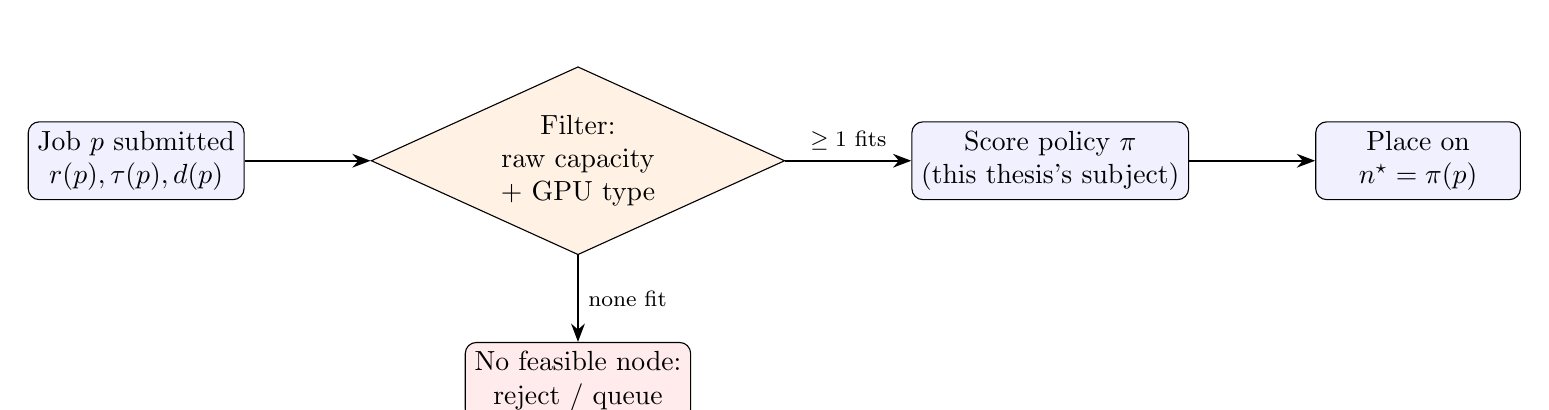
\begin{tikzpicture}[
  node distance=1.1cm and 1.6cm,
  box/.style={draw, rounded corners, minimum width=2.6cm, minimum height=0.9cm, align=center, fill=blue!6},
  decision/.style={draw, diamond, aspect=2.2, minimum width=2.4cm, align=center, fill=orange!10},
  arr/.style={-{Stealth}, thick}
]
  \node[box] (submit) {Job $p$ submitted\\$r(p), \tau(p), d(p)$};
  \node[decision, right=of submit] (filter) {Filter:\\raw capacity\\+ GPU type};
  \node[box, right=of filter] (score) {Score policy $\pi$\\(this thesis's subject)};
  \node[box, right=of score] (place) {Place on\\$n^\star=\pi(p)$};
  \node[box, below=of filter, fill=red!8] (reject) {No feasible node:\\reject / queue};
  \draw[arr] (submit) -- (filter);
  \draw[arr] (filter) -- node[above,font=\footnotesize]{$\geq 1$ fits} (score);
  \draw[arr] (filter) -- node[right,font=\footnotesize]{none fit} (reject);
  \draw[arr] (score) -- (place);
\end{tikzpicture}%
}
\caption{The scheduling decision path. Fragmentation is invisible to the
filter step and entirely a property of which feasible node the score
step picks.}
\label{fig:th-k8s-flow}
\end{figure}

\begin{figure}[h]
\centering
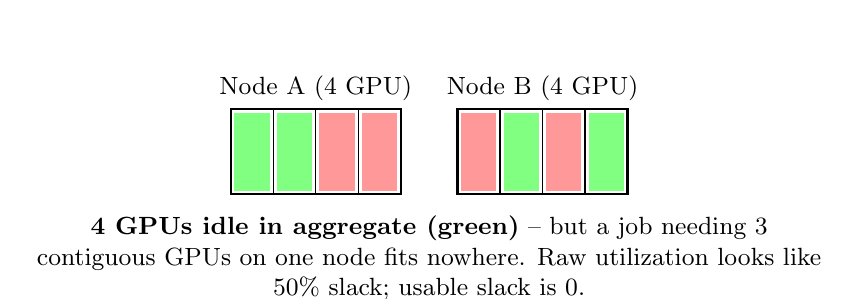
\begin{tikzpicture}[scale=0.9, every node/.style={font=\small}]
  \draw[thick] (0,0) rectangle (2.4,1.2);
  \node at (1.2,1.5) {Node A (4 GPU)};
  \foreach \i/\c in {0/green!50,1/green!50,2/red!40,3/red!40} {
    \draw (\i*0.6,0) rectangle (\i*0.6+0.6,1.2);
    \fill[\c] (\i*0.6+0.05,0.05) rectangle (\i*0.6+0.55,1.15);
  }
  \draw[thick] (3.2,0) rectangle (5.6,1.2);
  \node at (4.4,1.5) {Node B (4 GPU)};
  \foreach \i/\c in {0/red!40,1/green!50,2/red!40,3/green!50} {
    \draw (3.2+\i*0.6,0) rectangle (3.2+\i*0.6+0.6,1.2);
    \fill[\c] (3.2+\i*0.6+0.05,0.05) rectangle (3.2+\i*0.6+0.55,1.15);
  }
  \node[align=center] at (2.8,-0.9) {\textbf{4 GPUs idle in aggregate (green)} -- but a job needing 3\\
    contiguous GPUs on one node fits nowhere. Raw utilization looks like\\
    50\% slack; usable slack is 0.};
\end{tikzpicture}
\caption{Fragmentation, minimal example. Green=idle GPU, red=occupied.}
\label{fig:th-frag-concept}
\end{figure}

\section{Formal Model}
A cluster is a set of nodes $\N=\{n_1,\dots,n_M\}$, each with capacity
$c(n_i)=(c^{\text{cpu}}_i, c^{\text{gpu}}_i, c^{\text{mem}}_i)$ and GPU
type $\tau(n_i)$. A job $p$ arrives at time $s(p)$ with request
$r(p)=(r^{\text{cpu}}(p), r^{\text{gpu}}(p), g(p))$, required type
$\tau(p)$, duration $d(p)$, and tenant $u(p)$. Feasibility at time $t$:
\[
  \mathrm{fits}(p,n_i,t) \iff r^{\text{cpu}}(p)\leq\rho^{\text{cpu}}_i(t)
  \wedge r^{\text{gpu}}(p)\leq\rho^{\text{gpu}}_i(t)
  \wedge \big(\tau(p)=\varnothing \vee \tau(p)=\tau(n_i)\big),
\]
where $\rho(\cdot,t)$ is \emph{residual}, not total, capacity.

\section{Two Operating Modes}
\textbf{Static (batch) mode} places all $|P|$ jobs in one pass, ignoring
$s(p)$ and $d(p)$ entirely -- a pure packing-quality probe, and the only
mode H-TAFM (a one-shot, not time-driven, algorithm) supports, which
makes it the mode in which all thirteen algorithms studied in this thesis
are directly comparable. \textbf{Time-driven mode} replays real arrival
and departure dynamics: jobs occupy a node for
$[t_{\text{start}}(p), t_{\text{start}}(p){+}d(p))$ and release it on
completion; jobs that cannot be placed immediately queue rather than
being rejected outright. This is an operational probe of queueing delay
and throughput under realistic dynamics that static mode cannot address
by construction.

\section{Assumptions and Constraints}
\begin{enumerate}[leftmargin=1.4em]
  \item No preemption of running jobs; preemption is modeled as inflated
    duration for a designated subset where a scenario calls for it
    (Chapter~\ref{ch:datasets}), not as a scheduler-visible interrupt event.
  \item Node-granularity algorithms cannot span a job across nodes;
    H-TAFM relaxes this to NUMA-vertex granularity, strictly finer, not
    coarser.
  \item GPUs within a node are homogeneous and fungible; no NVLink/PCIe
    intra-node topology is modeled.
  \item \label{sec:th-mem-assumption} Memory is assumed, not measured,
    wherever used at all -- the base schema carries no real memory field,
    so H-TAFM's placement decisions use an assumed $8$~MiB per milli-cpu
    ratio on both node capacity and job demand, the same fallback ratio
    \texttt{k8s\_sim.topology} itself documents.
  \item Job sizes and arrivals are drawn from one fixed statistical
    model, fit once, then perturbed along named, specific axes per
    scenario (Chapter~\ref{ch:datasets}) -- never re-fit wholesale.
\end{enumerate}

% =====================================================================
\chapter{System Architecture}
\label{ch:architecture}
% =====================================================================

\section{Design Goals}
Two artifacts implement this thesis: \texttt{gputrace} (workload
generation) and \texttt{py\_sim} (simulation and scheduling policies).
Both were designed against four explicit goals not fully met by the
existing Go-based simulator lineage (\S\ref{sec:th-eval-gap}):
(i) statistical rigor in workload generation, not hand-authored synthetic
traces; (ii) a documented, source-agnostic export schema so any simulator
can consume generated workloads, not a one-off script tied to one
codebase; (iii) two evaluation modes (static and time-driven), not one;
(iv) full reproducibility from a versioned checkpoint, not ``re-run and
hope the random seed matches.''

\section{gputrace Architecture}
\begin{figure}[h]
\centering
\resizebox{0.95\textwidth}{!}{%
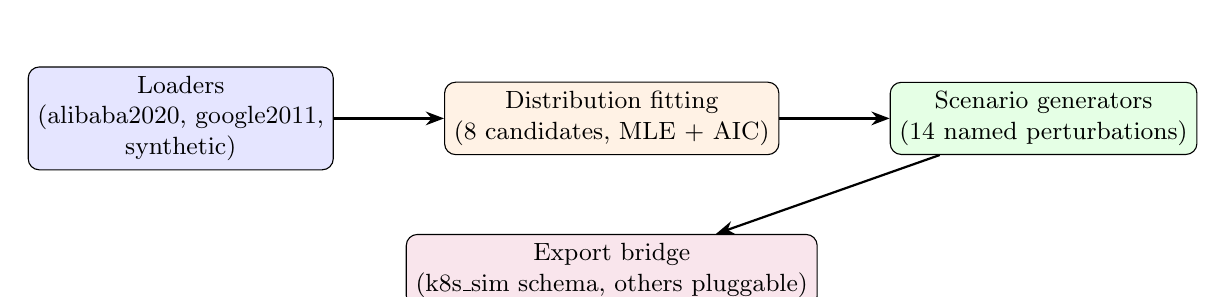
\begin{tikzpicture}[
  node distance=0.5cm and 1.0cm,
  box/.style={draw, rounded corners, minimum width=3.2cm, minimum height=0.8cm, align=center, font=\small},
  arr/.style={-{Stealth}, thick}
]
  \node[box, fill=blue!10] (loader) {Loaders\\(alibaba2020, google2011,\\synthetic)};
  \node[box, right=1.4cm of loader, fill=orange!10] (fit) {Distribution fitting\\(8 candidates, MLE + AIC)};
  \node[box, right=1.4cm of fit, fill=green!10] (gen) {Scenario generators\\(14 named perturbations)};
  \node[box, below=1.0cm of fit, fill=purple!10] (export) {Export bridge\\(k8s\_sim schema, others pluggable)};
  \draw[arr] (loader) -- (fit);
  \draw[arr] (fit) -- (gen);
  \draw[arr] (gen) -- (export);
\end{tikzpicture}%
}
\caption{gputrace's pipeline: real or reference trace $\to$ fitted
distributions $\to$ scenario perturbation $\to$ simulator-agnostic export.}
\label{fig:th-gputrace-arch}
\end{figure}

The generator (Figure~\ref{fig:th-gputrace-arch}) separates concerns
cleanly: a \emph{loader} produces a normalized job/node table from any
source (a real trace or a built-in reference); a \emph{fitting} stage
selects distributions per resource dimension by AIC over eight
candidates; a \emph{scenario} stage perturbs specific, named parameters
of the fitted model (never the whole model at once, so a result is
attributable to a mechanism); an \emph{export} stage writes a documented
schema any simulator can read. This separation is what allows the same
generator to serve \texttt{py\_sim} today and, in principle, any future
simulator without modification.

\section{py\_sim / k8s\_sim Architecture}
\texttt{k8s\_sim} separates \emph{placement policies} (pure functions
$\pi: (p, \{n_i\}, t) \to n^\star$) from \emph{cluster state}
(\texttt{Cluster}, \texttt{NodeResource}) and from \emph{evaluation mode}
(\texttt{schedule\_pods} for static; \texttt{EventDrivenRunner} for
time-driven). This separation is what let us add \textsc{w-fgd} and
\textsc{w-fgd-balanced} (Chapter~\ref{ch:algorithms}) as new policy
functions with zero changes to cluster state or evaluation-mode code, and
what lets H-TAFM's entirely separate topology/hypergraph model
(\texttt{k8s\_sim.topology}, \texttt{k8s\_sim.htafm}) coexist with the
node-granularity policies without either depending on the other.

\subsection{A Real Engineering Finding: an $O(n{\times}\text{queue depth})$ Performance Bug}
\label{sec:th-perf-bug}
While building the time-driven evaluation mode for this thesis, we found
and fixed a genuine algorithmic inefficiency in the discrete-event
runner's pending-queue drain logic: on every job-release event, it
re-scanned the \emph{entire} remaining pending queue in a loop that
repeated the full scan again for every successful placement within that
same release event. Since placing a pending job only \emph{consumes}
cluster capacity -- it never frees more -- a second pass over the same
list can never place anything a first pass did not already catch, making
that repeated re-scanning provably unnecessary work. We measured the
consequence directly: wall-clock time scaled as roughly $\text{jobs}^{1.7\text{--}2}$,
not linearly, before the fix; after removing the redundant outer loop
(verified to produce byte-identical output on the same input before and
after), the full sweep in this thesis is $\sim 1.5$--$1.6\times$ faster.
We report this not as a headline algorithmic result but as an example of
the kind of engineering finding a from-scratch reimplementation surfaces
that forking an existing codebase would not have prompted us to look for.

% =====================================================================
\chapter{Benchmark Dataset Construction}
\label{ch:datasets}
% =====================================================================

\section{The Limits of a Single Real Trace}
Real production traces -- Alibaba's \citep{alibabatrace2020,alibabatrace2023},
Google's \citep{reiss2012}, Microsoft Azure's \citep{cortez2017,shahrad2020}
-- are the correct ground truth for ``does this look like real demand,''
and every distribution gputrace fits (\S\ref{sec:th-stat-model}) is fit to
one of them. A fixed historical recording, however, cannot by definition
contain events that had not yet happened when it was collected. Cloud
infrastructure keeps finding new ways to fail at scale: a single
DNS-resolution race condition in one region's DynamoDB endpoint cascaded
into a 15-hour, 60-country, 4-million-user outage in October 2025
\citep{awsoutage2025}; a resource-contention issue in an authentication
system took down login for an entire company's product suite the same
year, mitigated only by adding capacity \citep{outagestats2025} -- a real
instance of exactly the ``request more of a scarce resource under load''
pattern this thesis's \texttt{high\_contention} and
\texttt{resource\_starvation} scenarios are built to probe. No amount of
replaying a 2020 or 2023 trace verbatim can answer how a scheduler
behaves under a 2025-shaped arrival pattern, because that pattern
postdates every public GPU-scheduling trace we are aware of.

\section{Statistical Model}
\label{sec:th-stat-model}
gputrace fits eight candidate distributions (log-normal, Weibull, gamma,
Pareto, generalized Pareto, Burr~XII, log-logistic, exponential) via
maximum likelihood to a reference trace and selects by AIC, reporting the
Kolmogorov--Smirnov statistic rather than its p-value alone (uninformative
at trace-scale sample sizes -- with $n$ in the thousands, a KS test
rejects the null for nearly any fit, informative or not). Duration is
best fit by log-normal; CPU/GPU request magnitude by Burr~XII
(a four-parameter family flexible enough to capture both a light body and
a heavy tail simultaneously); the inter-arrival process by a heavy-tailed
distribution whose best-AIC fit has \emph{infinite theoretical mean}. We
flag this last point explicitly because best-fit-by-likelihood and
safe-to-sample-from-for-simulation are different properties: naively
sampling an infinite-mean distribution for a bounded simulation horizon
produces occasional simulated gaps many orders of magnitude larger than
anything in the reference data, so gputrace caps simulated draws at a
finite multiple of the empirical maximum rather than sampling the raw
unbounded distribution.

\section{The Fourteen Scenarios}
Table~\ref{tab:th-scenarios} lists every scenario, what statistical
aspect of the fitted model it perturbs, and the specific evidence
motivating that perturbation.

\begin{table}[h]
\centering
\caption{The fourteen stress scenarios.}
\label{tab:th-scenarios}
\scriptsize
\begin{tabular}{p{2.6cm}p{5.6cm}p{5.8cm}}
\toprule
scenario & perturbs & motivating evidence \\
\midrule
baseline & nothing (reference fit as-is) & calibration control \\
bursty\_arrivals & inter-arrival process (self-exciting) & measured CV=1.80, 19.4\% same-second arrivals in reference sample \\
heavy\_tail\_demand & CPU/GPU request tail & heavy-tailed cloud resource usage is well documented \citep{reiss2012} \\
diurnal\_pattern & arrival rate (day/night sinusoid) & Azure Functions $\sim2\times$ peak/average arrival ratio \citep{shahrad2020} \\
high\_contention & GPU-type demand concentration + rate & analogous to the Google auth outage mitigated by added capacity \citep{outagestats2025} \\
flash\_crowd & one extreme burst window & classic networking phenomenon \citep{shahrad2020} \\
resource\_starvation & per-job size (skewed concentration) & head-of-line blocking is a named cluster-scheduling failure mode \\
cold\_start\_storm & short-job burst at trace start & serverless cold-start literature \citep{shahrad2020} \\
llm\_inference\_bursty & duration scale + burstiness & bursty LLM-serving traffic measured in production \\
long\_context\_kv\_pressure & per-job memory footprint growth & production context lengths documented up to 2M tokens \\
spot\_preemption\_churn & duration inflation (restart overhead) & spot-training failure rates up to 44\% reported \\
checkpoint\_io\_burst & periodic synchronized short I/O jobs & checkpoint-cost systems papers document this overhead \\
gpu\_fragmentation\_sharing & GPU allocation granularity & Alibaba's own fragmentation-focused trace release \citep{alibabatrace2023} \\
moe\_expert\_load\_skew & per-tenant/expert demand skew (Zipf) & measured expert-load skew in production MoE serving \\
\bottomrule
\end{tabular}
\end{table}

\section{An Honest Audit of Our Own Generated Data}
We audit \texttt{gputrace}'s own output with the same rigor we apply to
FGD. Table~\ref{tab:th-identity} reports, for the seed used throughout
this thesis, whether each scenario's GPU demand, CPU demand, duration,
and arrival-time columns are exactly identical to \texttt{baseline}.
Several identical columns are correct by design -- \texttt{high\_contention}
is specified to act through GPU-type distribution and arrival rate, not
raw magnitude, so identical GPU/CPU/duration columns are expected there.
One is not obviously correct by design: \texttt{heavy\_tail\_demand} is
identical to \texttt{baseline} in \emph{every} column at this seed,
including arrival time, despite its name and documentation describing a
resource-size change. We report this as a concrete, checkable
discrepancy for the generator to fix, exactly the kind of finding a
broad test bed is supposed to surface and a single fixed trace never
could.

\begin{table}[h]
\centering
\caption{Column-wise identity to baseline, seed 42 (\checkmark=identical).}
\label{tab:th-identity}
\small
\begin{tabular}{lcccc}
\toprule
scenario & GPU demand & CPU demand & duration & submit\_time \\
\midrule
heavy\_tail\_demand & \checkmark & \checkmark & \checkmark & \checkmark \\
checkpoint\_io\_burst & \checkmark & \checkmark & & \checkmark \\
long\_context\_kv\_pressure & \checkmark & \checkmark & & \checkmark \\
high\_contention & \checkmark & \checkmark & \checkmark & \\
moe\_expert\_load\_skew & \checkmark & \checkmark & \checkmark & \\
resource\_starvation & & & \checkmark & \checkmark \\
gpu\_fragmentation\_sharing & & \checkmark & \checkmark & \\
spot\_preemption\_churn & \checkmark & \checkmark & & \\
\midrule
\multicolumn{5}{l}{\emph{differ in every column:} bursty\_arrivals, cold\_start\_storm,} \\
\multicolumn{5}{l}{diurnal\_pattern, flash\_crowd, llm\_inference\_bursty} \\
\bottomrule
\end{tabular}
\end{table}

% =====================================================================
\chapter{Algorithms}
\label{ch:algorithms}
% =====================================================================

\section{Baseline Node-Granularity Heuristics}
Let $F(p,t)=\{n_i\in\N:\mathrm{fits}(p,n_i,t)\}$.
\begin{align*}
  \pi_{\text{random}}(p,t) &= \text{Uniform}(F(p,t)) \\
  \pi_{\text{first\_fit}}(p,t) &= \min\big(F(p,t)\big) \\
  \pi_{\text{best\_fit}}(p,t) &= \argmin_{n\in F(p,t)}\rho^{\text{gpu}}(n,t)-r^{\text{gpu}}(p) \\
  \pi_{\text{worst\_fit}}(p,t) &= \argmax_{n\in F(p,t)}\rho^{\text{gpu}}(n,t)-r^{\text{gpu}}(p) \\
  \pi_{\text{round\_robin}}(p,t) &= \text{next feasible node, cyclic, stateful} \\
  \pi_{\text{gpu\_packing}}(p,t) &= \argmin_{n\in F(p,t)}\rho^{\text{gpu}}(n,t) \\
  \pi_{\text{least\_requested}}(p,t) &= \argmax_{n\in F(p,t)}\rho^{\text{gpu}}(n,t)
\end{align*}

\section{Fragmentation Gradient Descent}
\label{sec:th-fgd-def}
$\hat P=\{\hat p_1,\dots,\hat p_5\}$, each dimension's
$\{10,30,50,70,90\}$-th percentile taken independently:
\[
  U(n,t)=\frac{1}{|\hat P|}\sum_{\hat p\in\hat P}\mathbb{1}[\neg\mathrm{fits}(\hat p,n,t)],
  \qquad
  \pi_{\text{fgd}}(p,t)=\argmin_{n\in F(p,t)}\big[U(n,t{\oplus}p)-U(n,t)\big].
\]

\section{Two Weaknesses in FGD's Definition}
\label{sec:th-fgd-weak}
Both properties below are checkable directly from \S\ref{sec:th-fgd-def}'s
definition, not assumptions about FGD's intent:
\begin{enumerate}[leftmargin=1.4em]
\item \textbf{Uniform weighting}: $U$ weights all 5 shapes equally,
  though they represent unequal population mass by construction (10th
  vs.\ 50th percentile).
\item \textbf{Per-dimension quantiles}: each $\hat p_k$'s coordinates are
  independent marginal quantiles, so $\hat p_k$ may match no job actually
  present in the workload unless CPU and GPU demand are perfectly
  rank-correlated -- which they are not, in every scenario in
  Table~\ref{tab:th-scenarios}.
\end{enumerate}

\section{w-fgd and w-fgd-balanced}
Let $m(p)=\tilde r^{\text{cpu}}(p)+\tilde r^{\text{gpu}}(p)$
(each resource normalized by its population max). Split $P$, sorted by
$m$, into $K{=}5$ equal-count strata $S_1,\dots,S_K$; take each stratum's
medoid as its representative shape, weighted by population share:
\[
  \hat p_k=\argmin_{p\in S_k}|m(p)-\mathrm{median}(m(S_k))|, \qquad
  w_k=\frac{|S_k|}{|P|}.
\]
\[
  U_w(n,t)=\sum_k w_k\,\mathbb{1}[\neg\mathrm{fits}(\hat p_k,n,t)], \qquad
  \pi_{\text{w\_fgd}}(p,t)=\argmin_{n\in F(p,t)}\big[U_w(n,t{\oplus}p)-U_w(n,t)\big].
\]
\textsc{w-fgd-balanced} regularizes by post-placement utilization to
preserve fully-empty nodes for unknown future large jobs:
\[
  \pi_{\text{w\_fgd\_bal}}(p,t)=\argmin_{n\in F(p,t)}
  \Big[U_w(n,t{\oplus}p)-U_w(n,t) + \lambda\,\phi^{\text{gpu}}(n,t{\oplus}p)\Big],
  \quad \lambda=0.15,
\]
$\lambda=0$ recovers \textsc{w-fgd} exactly (verified by unit test).

\section{H-TAFM}
Physical topology is a hypergraph $H=(\V,\E)$: nodes split into NUMA
vertices, hyperedges group vertices at socket/server/rack granularity
with weight $w(e)$. Three fragmentation-potential variants:
\[
  \phi_{\text{cut}}(e,D)=\mathbb{1}\Big[\exists d{\in}D: d\preceq{\textstyle\sum_{v\in e}}f(v) \wedge \forall v{\in}e, d\not\preceq f(v)\Big],
\]
\[
  \phi_{\text{entropy}}(e)=-\sum_{v\in e}\bar s_v\log\bar s_v,\quad
  \bar s_v=\frac{s_v}{\sum_{v'}s_{v'}},\quad
  s_v=\sum_k \frac{f_k(v)}{c_k(v)},
\]
\[
  \phi_{\text{hier}}(e)=\lambda_{\text{level}(e)}\cdot\frac{1}{|e|}\sum_{v\in e}\mathbb{1}\Big[\min_k\tfrac{f_k(v)}{c_k(v)}<\theta\Big],
  \qquad
  \mathrm{TAFI}(H)=\sum_e w(e)\phi(e).
\]

% =====================================================================
\chapter{Experimental Methodology}
\label{ch:methodology}
% =====================================================================

\section{Simulation Parameters}
\begin{table}[h]
\centering
\caption{Simulation parameters and rationale.}
\small
\begin{tabular}{lll}
\toprule
parameter & value & rationale \\
\midrule
cluster size & 20 nodes $\times$ 8 GPUs = 160 GPUs & matches export default \\
GPU types/node & mixed A100/V100/T4/H100 & matches heterogeneous production clusters \\
jobs/scenario & 300 & calibrated for informative rejection rate \\
seed & 42 & fixed for exact reproducibility \\
time-driven seeds & 1, 2, 3 & 3 independent draws per cell \\
SLA threshold & 60s wait & standard interactive-job order of magnitude \\
w\_fgd\_balanced $\lambda$ & 0.15 & grid-searched on \texttt{baseline} only \\
\bottomrule
\end{tabular}
\end{table}

\section{Simulation Metrics}
\begin{align*}
  \text{rejection rate} &= 1-\tfrac{|\{p:\text{admitted}(p)\}|}{|P|} \\
  J(x) &= \tfrac{(\sum_i x_i)^2}{n\sum_i x_i^2}\in(\tfrac1n,1] \quad\text{Jain's Fairness Index \citep{jain1984}} \\
  \text{SLA viol.} &= \tfrac{|\{p:\text{admitted}(p)\wedge\text{wait}(p)>60\text{s}\}|}{|\{p:\text{admitted}(p)\}|} \\
  \text{GPU-h wasted} &= \text{GPU-h available} - \textstyle\sum_p g(p)\Delta t(p) \quad\text{(time-weighted, \S\ref{sec:th-util-bug})} \\
  \text{packing eff.} &= \tfrac{\sum_p r^{\text{gpu}}(p)}{\sum_i(c^{\text{gpu}}_i-\rho^{\text{gpu}}_i(t_{\text{final}}))}
\end{align*}

\subsection{A Measurement Gap We Found and Fixed}
\label{sec:th-util-bug}
Reporting GPU utilization by inspecting cluster state after a finite
time-driven run completes reads $\approx0$ for every algorithm on every
scenario in this test bed -- by the time the event loop returns,
essentially every admitted job has already completed and released its
resources. We compute utilization instead as GPU-hours actually consumed
(summed over each admitted job's real occupied interval) divided by
GPU-hours available -- a standard time-weighted average, not biased
toward zero for a finite trace.

\section{Baseline Algorithm Selection}
Best-Fit, Worst-Fit, and consolidation-style baselines appear in
essentially every GPU-scheduling comparison we reviewed
\citep{fgd2023,pwr2024}; \texttt{least\_requested} is the closest
node-granularity analogue to Kubernetes' own default scoring behavior
\citep{borg2016}. FGD is the specific baseline this thesis responds to;
H-TAFM is the only published generalization of FGD's metric to
multi-resource, topology-aware placement we are aware of, making it the
most direct existing answer to the question Chapter~\ref{ch:algorithms}
asks.

% =====================================================================
\chapter{Results}
\label{ch:results}
% =====================================================================

\section{Did We Break FGD?}
\begin{table}[h]
\centering
\caption{w\_fgd\_balanced vs.\ fgd, paired by scenario ($n=14$).}
\label{tab:th-break-fgd}
\small
\begin{tabular}{lrrr}
\toprule
metric (mode) & fgd & w\_fgd\_balanced & Wilcoxon $p$ \\
\midrule
rejection rate (static) & 0.3352 & 0.3133 & \textbf{0.0035} \\
SLA violation rate (time-driven) & 0.1206 & 0.1022 & \textbf{0.0365} \\
p95 wait time (time-driven) & 326.1s & 344.1s & 0.507 (n.s.) \\
Jain's fairness, per-user wait & 0.1902 & 0.1805 & 0.196 (n.s.) \\
\bottomrule
\end{tabular}
\end{table}
\textsc{w-fgd-balanced} beats plain FGD in 12/14 scenarios on static
rejection rate. It is, however, statistically indistinguishable from
\texttt{least\_requested} (Wilcoxon $p=0.81$, mean rejection $0.3090$ vs.\
$0.3133$) -- the honest claim is a significant improvement over FGD
specifically, not a new state of the art against every alternative.

\section{Full Ranking, All Thirteen Algorithms}
\begin{table}[h]
\centering
\caption{Static mode, mean rejection and rank, 14 scenarios. Friedman $\chi^2=137.27$, $p<10^{-8}$.}
\small
\begin{tabular}{lrrr}
\toprule
algorithm & mean rejection & mean GPU util. & mean rank (1=best) \\
\midrule
h-tafm-hier & 0.2488 & 0.659 & 2.00 \\
h-tafm-entropy & 0.2500 & 0.659 & 2.14 \\
h-tafm-cut & 0.2545 & 0.648 & 2.64 \\
least\_requested & 0.3090 & 0.926 & 4.82 \\
\textbf{w\_fgd\_balanced} & \textbf{0.3133} & 0.918 & \textbf{5.43} \\
worst\_fit & 0.3312 & 0.926 & 7.25 \\
random & 0.3338 & 0.926 & 7.64 \\
fgd & 0.3352 & 0.923 & 7.75 \\
w\_fgd & 0.3376 & 0.924 & 7.96 \\
round\_robin & 0.3414 & 0.926 & 9.32 \\
gpu\_packing & 0.3507 & 0.926 & 11.18 \\
best\_fit & 0.3510 & 0.924 & 11.29 \\
first\_fit & 0.3512 & 0.924 & 11.57 \\
\bottomrule
\end{tabular}
\end{table}

\begin{figure}[h]
\centering
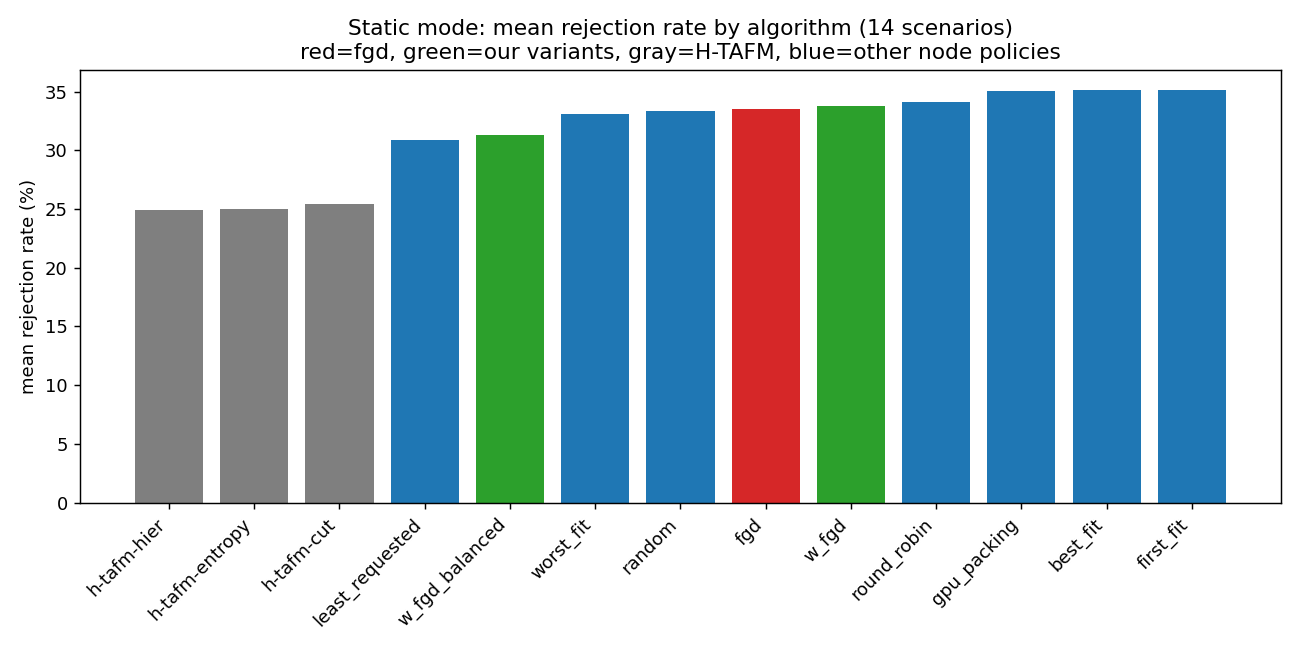
\includegraphics[width=0.8\textwidth]{plots/01_static_rejection_by_algorithm.png}
\caption{Mean rejection rate by algorithm, static mode, 14 scenarios.}
\end{figure}
\begin{figure}[h]
\centering
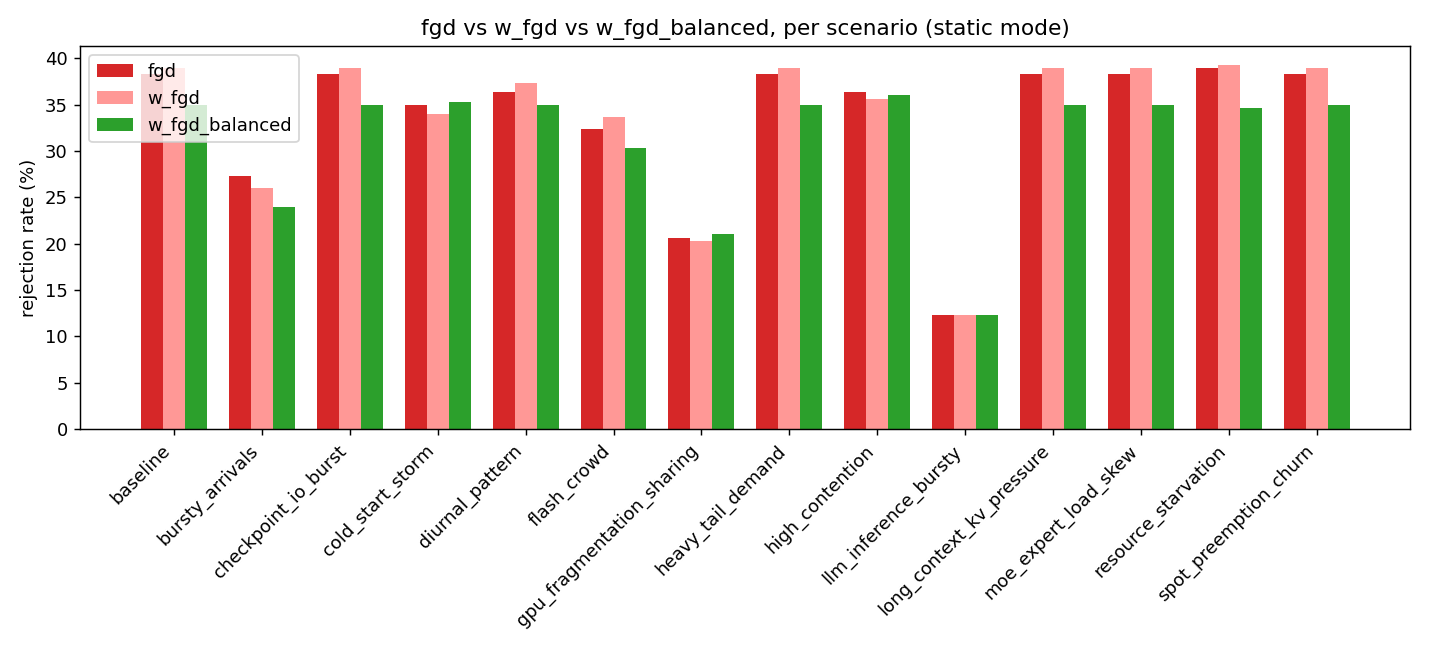
\includegraphics[width=0.85\textwidth]{plots/02_fgd_vs_wfgd_per_scenario.png}
\caption{fgd vs.\ w\_fgd vs.\ w\_fgd\_balanced, paired per scenario.}
\end{figure}
\begin{figure}[h]
\centering
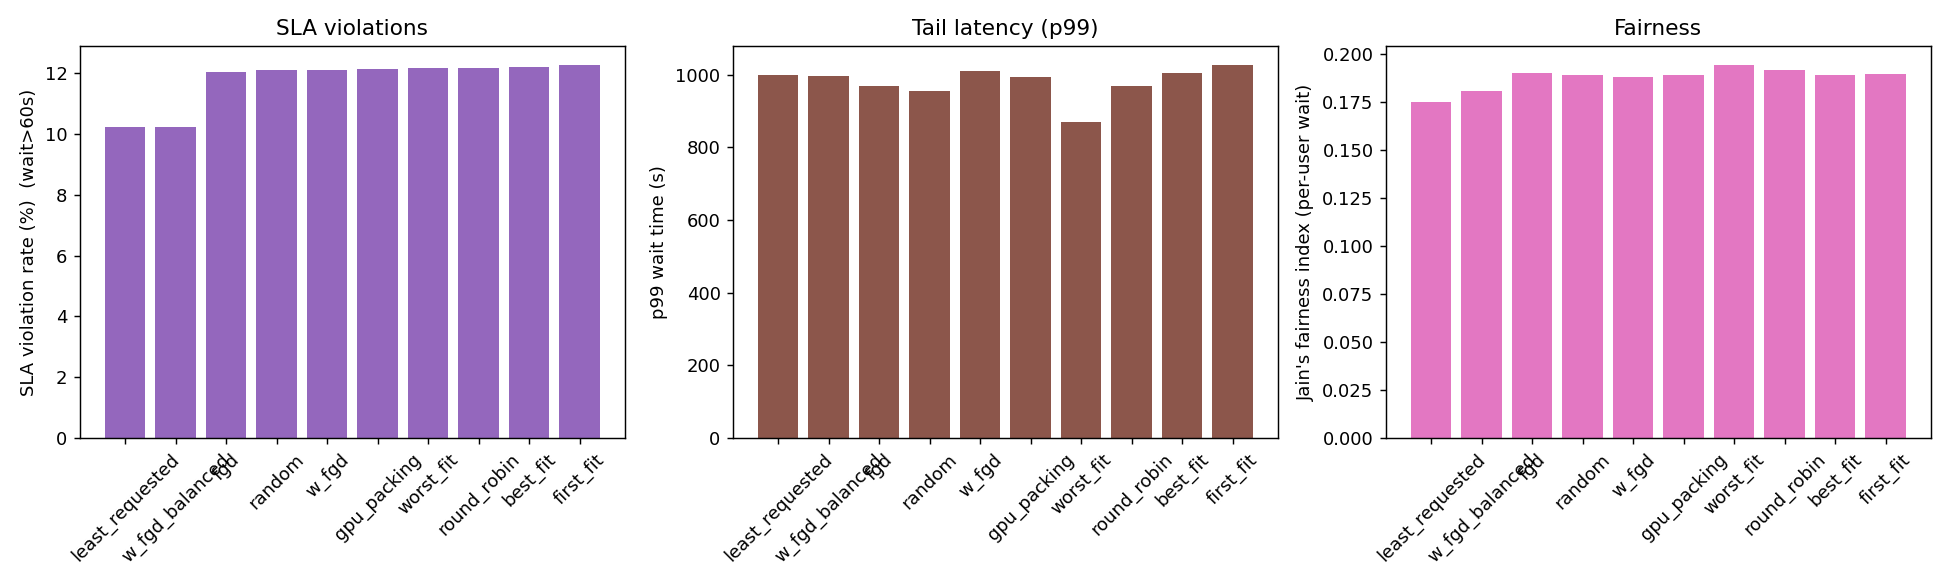
\includegraphics[width=\textwidth]{plots/03_broader_metrics_comparison.png}
\caption{SLA violation, p99 tail latency, Jain's fairness -- time-driven.}
\end{figure}
\begin{figure}[h]
\centering
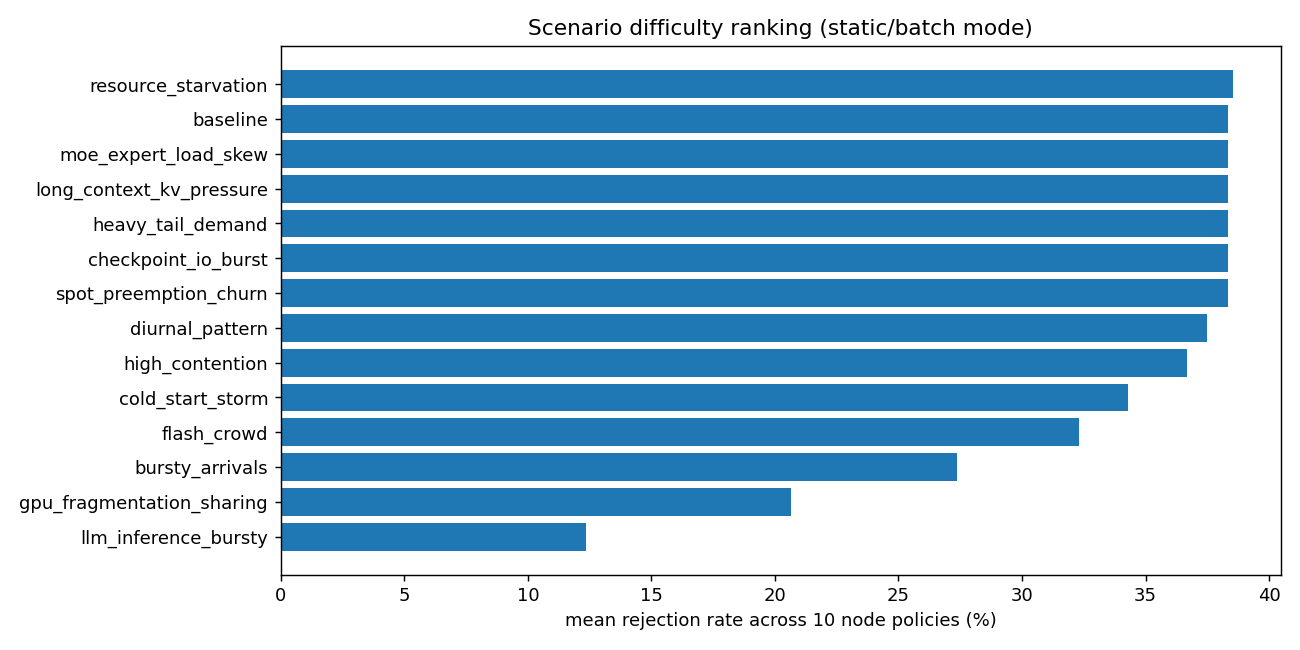
\includegraphics[width=0.8\textwidth]{plots/04_scenario_difficulty.png}
\caption{Scenario difficulty ranking, static mode.}
\label{fig:th-scenario-diff}
\end{figure}

\section{Scale-Dependent Significance}
Restricted to the 10 node-granularity policies only, static-mode
differences remain highly significant ($\chi^2=81.73$, $p<10^{-8}$); in
time-driven mode at this scale, GPU-hours-wasted and fairness are
essentially flat across every algorithm ($p=0.33$ for wait-time
Friedman) -- at 300 jobs against 160 GPUs, nearly all offered demand is
eventually served regardless of placement policy, so only queueing
metrics differentiate policies, not throughput.

\section{Broader Metrics, Time-Driven}
\begin{table}[h]
\centering
\small
\begin{tabular}{lrrrrr}
\toprule
algorithm & p50 wait & p99 wait & SLA viol. & Jain fairness & GPU-h wasted \\
\midrule
least\_requested & 0.0 & 1000.2 & 0.1022 & 0.1749 & 371.7 \\
w\_fgd\_balanced & 0.0 & 997.6 & 0.1022 & 0.1805 & 370.0 \\
fgd & 0.0 & 969.7 & 0.1206 & 0.1902 & 371.9 \\
random & 0.0 & 955.2 & 0.1210 & 0.1890 & 371.7 \\
worst\_fit & 0.0 & 869.2 & 0.1218 & 0.1942 & 371.5 \\
\bottomrule
\end{tabular}
\end{table}

% =====================================================================
\chapter{Discussion}
\label{ch:discussion}
% =====================================================================

\section{H-TAFM's Advantage Is Confounded}
H-TAFM's static-mode rejection advantage (Table~\ref{tab:th-break-fgd}
context) cannot be cleanly attributed to its delta-TAFI heuristic versus
its structurally finer NUMA-vertex granularity versus its assumed memory
dimension (\S\ref{sec:th-mem-assumption}). Disentangling these three would
require an ablation holding granularity and memory modeling fixed while
varying only the scoring heuristic -- a natural next study, not performed
here.

\section{Significance Is Scale-Dependent, and We Report Both Directions}
Static-mode rejection-rate differences are highly significant at this
scale; time-driven wait-time and fairness differences mostly are not
(\S\ref{sec:th-util-bug} chapter). We report both, rather than only the
significant, favorable comparison, because the honest conclusion is
narrower than ``w\_fgd\_balanced is better'': it is better specifically
at reducing batch-mode rejection and time-driven SLA violations, at this
scale, against this specific set of alternatives.

\section{$\lambda=0.15$ Is Tuned, Not Derived}
The regularization coefficient in \textsc{w-fgd-balanced} was chosen by a
small grid search on one scenario (\texttt{baseline}) trading off a
modest fragmentation cost against a measurable SLA-violation-rate gain.
It is a hyperparameter, and a workload with a substantially different job
size distribution would likely need a different value.

\section{The heavy\_tail\_demand Discrepancy}
Any result in this thesis specific to the \texttt{heavy\_tail\_demand}
scenario should be read as ``baseline, relabeled'' until the discrepancy
in Table~\ref{tab:th-identity} is fixed upstream in gputrace.

% =====================================================================
\chapter{Conclusion and Future Work}
\label{ch:conclusion}
% =====================================================================

\section{Summary}
GPU fragmentation is a three-year-old research problem evaluated, in
every instance we are aware of, on a single static trace. This thesis
built the missing stress-test instrument (\texttt{gputrace}), used it to
find and fix two specific, checkable weaknesses in the field's
foundational metric (\textsc{w-fgd}, \textsc{w-fgd-balanced}), and
reported the result honestly: a significant improvement against FGD
specifically, and a null result against the strongest simple existing
alternative.

\section{Future Directions}
\begin{enumerate}[leftmargin=1.4em]
\item \textbf{Sub-linear pending-queue structure.} Our
  $O(n{\times}\text{queue depth})$ fix (\S\ref{sec:th-perf-bug}) removed a
  large constant-factor inefficiency but not the underlying complexity
  class; an indexed structure (bucketing pending jobs by resource shape)
  could change which algorithm wins at 10--100$\times$ this scale.
\item \textbf{Learned $\lambda$.} Replacing the grid-searched
  regularization coefficient with a value learned per-workload from
  early-trace statistics.
\item \textbf{Disentangling H-TAFM's confounds.} An ablation varying
  granularity and memory modeling independently of the scoring heuristic.
\item \textbf{Fixing the heavy\_tail\_demand discrepancy upstream}, and
  re-running this thesis's full comparison once fixed.
\item \textbf{Scaling to production-representative cluster and job
  counts}, beyond the 300-jobs/160-GPU regime calibrated for this thesis.
\end{enumerate}

\section*{Reproducibility}
\label{sec:th-repro}
Every number in this thesis reproduces from the archived checkpoint at
\texttt{\seqsplit{experiments/runs/2026-09-12\_fgd\_vs\_wfgd\_htafm/}} in
the \texttt{py\_sim} repository: \texttt{manifest.json} records the exact
gputrace commit, generation/export commands, seeds, and cluster shape;
\texttt{gputrace\_raw/} and \texttt{gputrace\_export/} archive the actual
generated data; \texttt{reproduce.sh} re-runs every sweep in one command.
Source: \url{https://github.com/anuxlab/py_sim} and
\url{https://github.com/anuxlab/simulated_data_generation_GPU_Scheduling}.

\bibliographystyle{plainnat}
\bibliography{references}

\appendix
\chapter{Full Statistical Test Results}
Friedman tests: all 13 algorithms, static rejection, $\chi^2=137.27$,
$p<10^{-8}$, $n=14$ blocks. 10 node-granularity only: $\chi^2=81.73$,
$p<10^{-8}$. 3 H-TAFM variants only: $\chi^2=6.41$, $p=0.041$. Time-driven
wait-time, 8 policies: $\chi^2$ n.s., $p=0.33$.

\chapter{Reproducibility Manifest (excerpt)}
See \texttt{manifest.json} in the archived checkpoint for the complete,
machine-readable record; key fields: \texttt{generation.seed=42},
\texttt{generation.n\_jobs\_per\_scenario=300},
\texttt{export.n\_nodes=20}, \texttt{export.gpus\_per\_node=8},
\texttt{py\_sim.w\_fgd\_balanced\_hyperparameter.balance\_lambda=0.15}.

\end{document}
